\chapter{显示器面板参数}
论文中提及的显示器面板参数。

在面板的参数中,我们重点关注其尺寸及PPI、面板亮度、工作频率、面板类型以及反应时间。

\begin{figure}[!htbp]
\centering
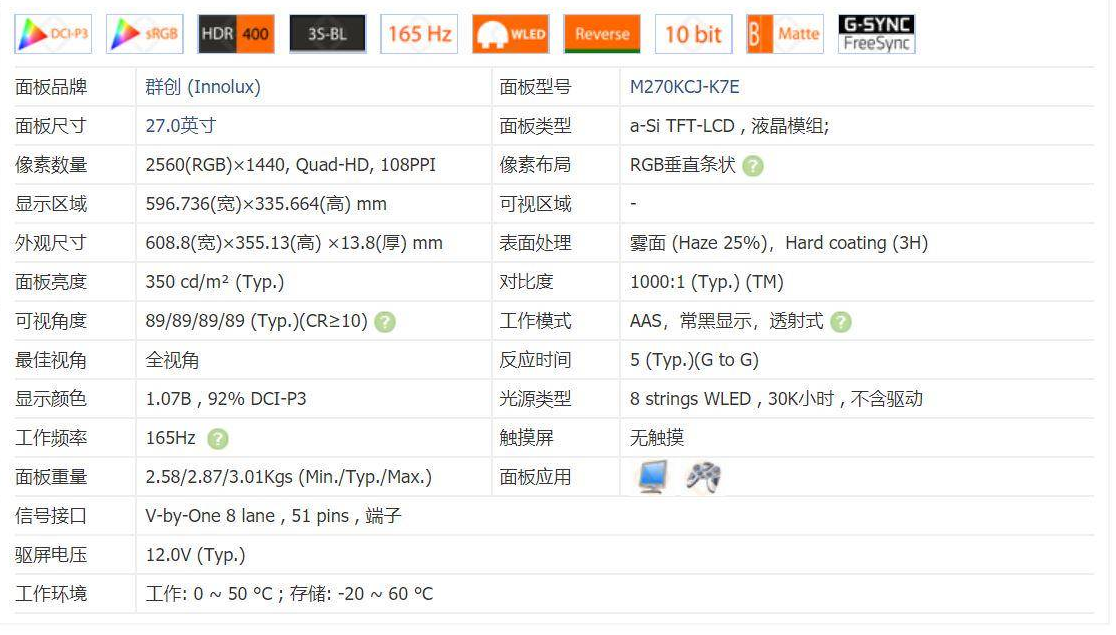
\includegraphics[scale=0.5]{figures/HW/PA_A.png}
\caption{AOCQ27G2S-K7E面板}
\end{figure}

\begin{figure}[!htbp]
\centering
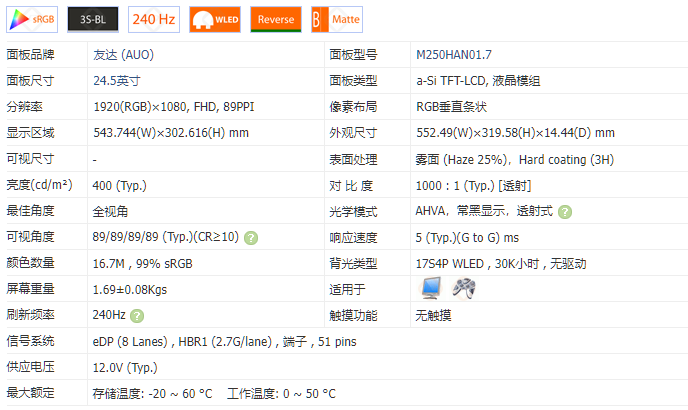
\includegraphics[scale=0.8]{figures/HW/PA_B.png}
\caption{BENQXL2546K面板}
\end{figure}

\begin{figure}[!htbp]
\centering
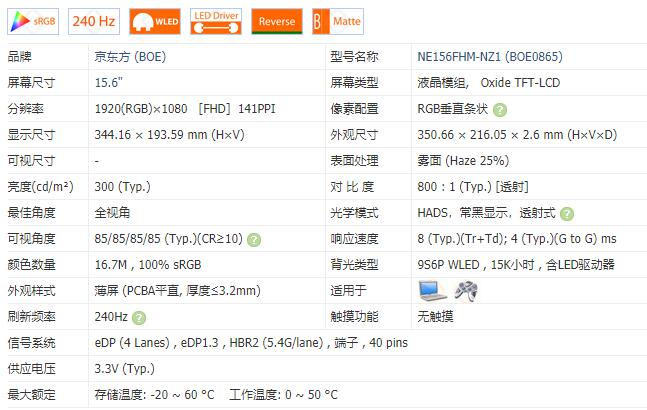
\includegraphics[scale=0.8]{figures/HW/PA_C.png}
\caption{BOENE156FHM-NZ1面板}
\end{figure}

\chapter{前后端接口列表}
前后端对接所依赖的接口列表。

NTP相关

同步NTP时间
0.0.0.0:8000/DecoderBack/NtpSync/

参数:
ip: NTP服务器IP或URL(ntp.aliyun.com),
time-zone: 时区('Asia/Shanghai'),
返回:
isOk: 执行状况(True/False),

网络接口相关

获取管理接口配置与状态
0.0.0.0:8000/DecoderBack/GetManagePortConfig/

参数:无参数

返回:
isOk: 执行状况(True/False),
managemenmtPortConfig: 管理接口配置,

获取业务接口配置
0.0.0.0:8000/DecoderBack/GetDataPortConfig/

参数:无参数,

返回:
isOk: 执行状况(True/False),
dataPortConfig: 业务接口配置,

获取网口配置
0.0.0.0:8000/DecoderBack/GetEthernetPortConfig/

参数:无参数,

返回:
isOk: 执行状况(True/False),
dataPortConfig: 网口配置,

编辑管理接口配置[仅数据库]
0.0.0.0:8000/DecoderBack/EditManagePortConfig/

参数:
ip,
port,
subnet-mask 子网掩码,
gateway 网关,
status 链路状态(bool),
web-running Web服务运行状态(bool),
ping-allowance 允许ping(bool),

返回:
操作状态,

编辑业务接口配置[仅数据库]
0.0.0.0:8000/DecoderBack/EditDataPortConfig/

参数:
access 对应编码端网口,
exit-access 对应解码端网口,
exit-port 出口端口,
target-ip = 目的ip,
target-port = 目的端口,
protocol = 协议,

返回:
操作状态,

编辑网口配置[仅数据库]
0.0.0.0:8000/DecoderBack/EditEthernetPortConfig/

参数:
ip 网口IP,
access 网口号,
subnet-mask 子网掩码,
gateway 网关,

返回:
操作状态,
系统状态相关,

获取系统状态
0.0.0.0:8000/DecoderBack/GetSystemStatus/

参数:无参数,

返回:CPU, RAM,存储,

IP白名单相关

获取IP白名单列表
0.0.0.0:8000/DecoderBack/GetIpWhiteList/

参数:
offset 日志展示起始位置,[offset : offset+20],

返回:
IP白名单列表,

新增IP白名单项
0.0.0.0:8000/DecoderBack/AddIpWhiteList/

参数:
ip: 新增IP,

返回:
操作状态,

删除IP白名单项
0.0.0.0:8000/DecoderBack/DelIpWhiteList/

参数:
id: 白名单序列号(由GetIpWhiteList/返回),

返回:
操作状态,

编辑IP白名单项
0.0.0.0:8000/DecoderBack/EditIpWhiteList/

参数:
ip: 新增IP,
id: 白名单序列号(由GetIpWhiteList/返回),

返回:
操作状态,

用户相关

新增用户
0.0.0.0:8000/DecoderBack/AddUser/

参数:
account,
name,
password,
authority 权限 1=管理员 2=配置 3=审计,
active 活跃状态,

返回:
操作状态,

删除用户
0.0.0.0:8000/DecoderBack/DelUser/

参数:
account,

返回:
操作状态,

编辑用户
0.0.0.0:8000/DecoderBack/EditUser/

参数:
id,
account,
name,
password,
authority 权限 1=管理员 2=配置 3=审计,

返回:
操作状态,

获取用户列表
0.0.0.0:8000/DecoderBack/GetUserList/

参数:无参数,

返回:
用户列表,

获取用户信息(获取用户列表的单用户版本)
0.0.0.0:8000/DecoderBack/GetUserInfo/

参数:
account: 用户帐号,

返回:用户信息,

验证登录
0.0.0.0:8000/DecoderBack/AuthUser/

参数:
account: 用户帐号,
password: 用户密码 ,

返回:
能否登录,是否可管理,是否可查看,是否被冻结,

获取冻结名单
0.0.0.0:8000/DecoderBack/GetFreezingUserList/

返回:
冻结用户信息,

解冻用户
0.0.0.0:8000/DecoderBack/UnfreezeUser/

参数:
account: 用户帐号,

返回:
操作结果,

日志相关

获取日志列表
0.0.0.0:8000/DecoderBack/GetLog/

参数:
time-start: 筛选开始时间 2022-06-11 12:00:00[.123456],
time-end: 筛选结束时间,
classify: 日志类别(system, user, operation, warning)(''=All),
level: 日志级别(info, warning,) [''=all],
content 内容关键字筛选(''=All),
offset 日志展示起始位置,[offset : offset+20],

返回:
totalLength: 日志总条数,
Log: 可迭代,[[<时间>, <级别>, <内容>], [], []...],

传输相关

获取传输列表
0.0.0.0:8000/DecoderBack/GetTransferList/

参数:
time-start: 筛选开始时间,
time-end: 筛选结束时间,
exit-ip: 出口IP(''=All),
target-ip 目的IP(''=All),
protocol: 协议(''=All),
offset 日志展示起始位置,[offset : offset+20],

返回:
传输列表,

传输状态统计
0.0.0.0:8000/DecoderBack/GetTransferInfo/

参数:
time-start: 筛选开始时间,
time-end: 筛选结束时间,
Access: 网口选择(''=All),
protocol: 协议(''=All),

返回:
length: 数据条数,
size: 数据大小(字节数),

Token相关

Token会在AuthUser接口获得,这也是唯一一个无需token验证的接口。
在后续请求中,在Header部分加入Token,完成后续验证。

Token验证失败返回HTTP状态码401UnAuthorized

Messige释义:

No authenticate header:Header没有包含Authorization字段

Error authenticate header:Header包含Authorization字段,但无效或为空值

Token expired:token超过有效期限

Invalid token:无效的token

Unexpected token error:解析token时出现的其他错误

User no longer exist or token lost effiency:用户不再存在,或者被手动注销

Mismatched Authority: ManagementRight required:需要管理权限(但没有)

Mismatched Authority: AuditRight required:需要审计权限(但没有)
